\section{Datu izgūšana no ziņu portāliem ar rāpuli}
Lai veiktu izpēti, sakumā ir nepieciešams ievākt treniņdatus / valodas korpusu, kas raksturo problēmvidi – ziņu portālu rakstus. Praktiskai rāpuļa implementācijai tika izvēlēts Python ietvars “Scrapy”, ar kura palīdzību iespējams izveidot tīmekļa rāpuļus, kas pārmeklē mājaslapas un izvelk no tām datus strukturētā formā. Šis ietvars izvēlēts, jo tas ir viens no populārākajiem rīkiem šajā kategorijā un tas labi spēj apstrādāt un formatēt lielu datu apjomu. Tā kā tīmekļa rāpuļi ir jāpielāgo konkrētai mājaslapas struktūrai, lai iegūtu vēlamos datus, tika izvēlēts konkrēts portāls - delfi.lv, dēļ tā daudzveidīgā kategoriju klāsta un rakstu daudzuma. Darba ietvaros izveidots rāpulis, kas ievāc datus no šī portāla un saglabā tos JSON formā ar 4 pamatlaukiem – virsraksts, kategorija, saturs, hipersaite. Lai sašaurinātu problēmvidi un ierobežotu nepieciešamos resursus tika izvēlētas 5 apskatāmās kategorijas – kriminālziņas, biznesa, izklaides, politikas un sporta ziņas. Izgūta raksta piemēru JSON formātā iespējams apskatīt \ref{appendix:raksta_piemers} pielikumā.

Rezultātā tika ievākti 6526 raksti ar sadalījumu pa kategorijām kāds redzams tabulā \ref{tab:rakstu_kategorijas}
\begin{table}[H]
\centering
\caption{\label{tab:rakstu_kategorijas}}
\textbf{Ievākto rakstu sadalījums pa kategorijām\\}
\begin{tblr}{
  hlines,
  vlines,
}
Kategorija    & Raksti  \\
politika     & 1633   \\
kriminālziņas & 1286   \\
izklaide     & 1261   \\
sports       & 1180  \\
bizness      & 1166  
\end{tblr}
\end{table}

Ievācot rakstus novērots, ka bez rakstu satura atšķiras arī vidējie rakstu garumi katrā kategorijā. Politikas un biznesa ziņām raksturīgi gari raksti ar vidēji vairāk nekā 350 vārdiem, savukārt izklaides, sporta un kriminālziņām – krietni īsāki raksti (īpaši kriminālziņām ar vidējo rakstu garumu ap 115 vārdiem). Šāda atšķirība garumos varētu atstāt ietekmi uz konkrētu kategoriju klasifikāciju akurātumu. Rakstu iedalījumu garumos sīkāk iespējams apskatīt \ref{appendix:kategorijas_wc} pielikumā.

\section{Tekstu priekšapstrāde}
\subsection{Stopvārdu atmešana}
Izmantotajās Python bibliotēkās ir iekļauti saraksti ar stopvārdiem daudzām izplatītām valodām, tomēr latviešu valodai šāds sarakts jādefinē neatkarīgi. Tika veikta izpēte par to vai šāds saraksts jau ir publiski pieejams un kā viens no populārākajiem atrasts ‘stopwords-lv’ repozitorijs iekš github. Lai gan tas ir izmantojams kā labs pamats un uzskaita palīgvārdus (saikļus, prievārdus, partikulas), trūkst citas svarīgas morfoloģiskās grupas kā vietniekvārdi (attieksmes vietniekvārdi – kurš, kura u.c., norādāmie vietniekvārdi – šis, šī, tas, tā, viņš u.c, kā arī locījumi šiem vārdiem), jo arī šo vārdu esamība neraksturo teksta fragmenta jēgu vai piederību kādai kategorijai. Darba ietvaros izveidots uzlabots stopvārdu saraksts latviešu valodai, kas labāk spētu veikt vārdu filtrēšanas soli teksta priekšasptrādē, un pielietots uz apmācības datiem. 

\clearpage

\section{Algoritmu rezultāti}
\subsection{Atbalsta vektora mašīnas}

Atbalsta vektora mašīnas apmācības algoritms ir implementēts ar scikit-learn SVM klases komponenti LinearSVC (sklearn.svm.LinearSVC). Sasniegtais akurātums ar testa rakstu kopu un izmantojot vārdu maisa vektorizācijas pieeju -  0.952, pielietojot TF-IDF pazīmju izveidē savukārt tiek iegūts augstāks akurātums - \textbf{0.966}. Kā redzams pārpratuma matricā \ref{fig:AVM_TFIDF} - piecu kategoriju klasifikācija tiek veikta ļoti precīzi un biežākā kļūda ir nepareizi klasificētas politikas ziņas, klasificējot tās kā biznesa ziņas. Precīzāki novērtējumi pa kategorijām apskatāmi \ref{tab:AVM} tabulā.

\begin{figure}[H]
	\centering
	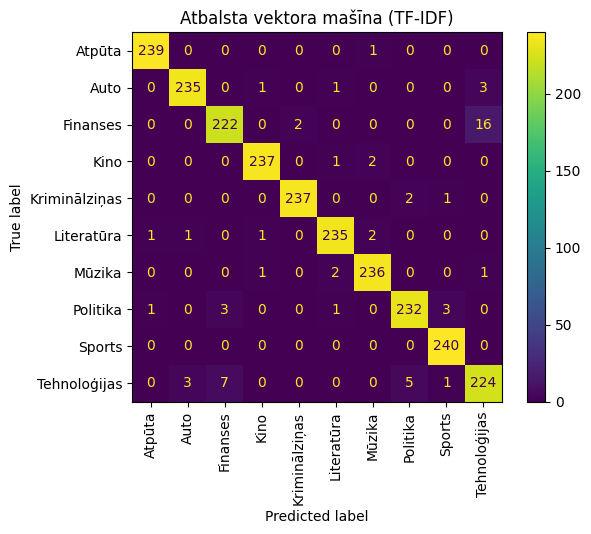
\includegraphics[width=0.75\textwidth]{AVM_TFIDF}
	\caption{Atbalsta vektora mašīnas pārpratuma matrica}
	\label{fig:AVM_TFIDF}
\end{figure}
\begin{table}[H]
\centering
\caption{\label{tab:AVM}}
\textbf{AVM algoritma novērtējums pa kategorijām\\}
\begin{tblr}{
  hlines,
  vlines,
}
kategorija & precizitāte & pārklājums   & F1 mērs \\
bizness  & 0.938017  & 0.970085 & 0.953782     \\
criminal & 0.979339  & 0.979339 & 0.979339     \\
izklaide & 0.98855   & 0.992337 & 0.99044     \\
politika & 0.965944  & 0.945455 & 0.95559     \\
sports   & 1         & 0.991632 & 0.995798     
\end{tblr}
\end{table}

\subsection{Naivā Bajesa metode}
TBD
\begin{figure}[H]
	\centering
	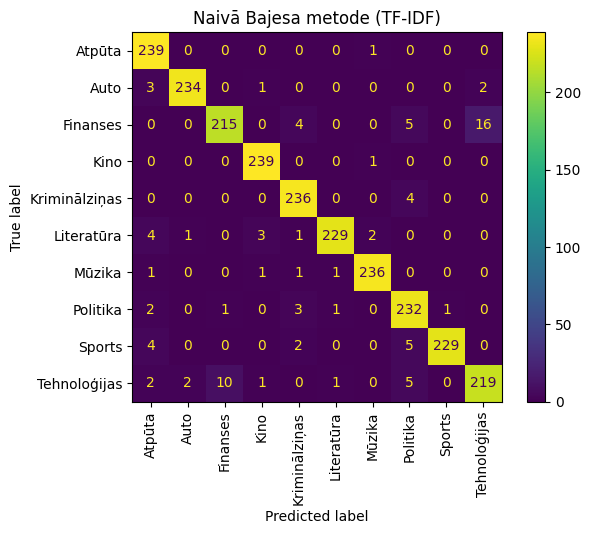
\includegraphics[width=0.75\textwidth]{NB_TFIDF}
	\caption{Naivā Bajesa metode pārpratuma matrica}
	\label{fig:NB_TFIDF}
\end{figure}
\begin{table}[H]
\centering
\caption{\label{tab:NB}}
\textbf{Naivā Bajesa algoritma novērtējums pa kategorijām\\}
\begin{tblr}{
  hlines,
  vlines,
}
kategorija & precizitāte & pārklājums   & F1 mērs \\
bizness  & 0.944724  & 0.803419 & 0.86836     \\
criminal & 0.982063  & 0.904959 & 0.941935     \\
izklaide & 0.995984  & 0.950192 & 0.972549     \\
politika & 0.794045  & 0.969697 & 0.873124     \\
sports   & 0.99569   & 0.966527 & 0.980892     \\
\end{tblr}
\end{table}

\subsection{Loģistiskā regresija}
TBD
\begin{figure}[H]
	\centering
	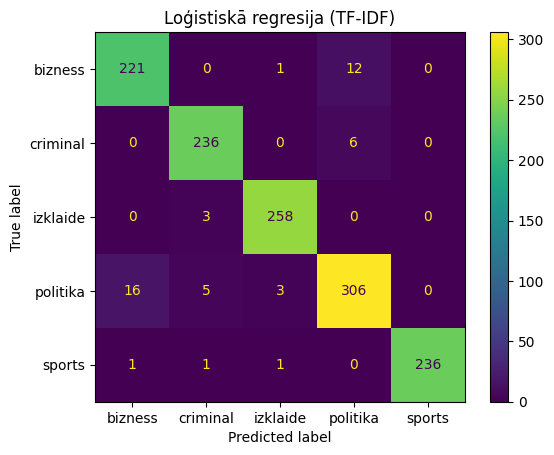
\includegraphics[width=0.75\textwidth]{LogRef_TFIDF}
	\caption{Loģistiskās regresijas pārpratuma matrica}
	\label{fig:LogRef_TFIDF}
\end{figure}
\begin{table}[H]
\centering
\caption{\label{tab:LogRef}}
\textbf{Loģistiskā regresijas algoritma novērtējums pa kategorijām\\}
\begin{tblr}{
  hlines,
  vlines,
}
kategorija & precizitāte & pārklājums   & F1 mērs \\
bizness  & 0.928571  & 0.944444 & 0.936441      \\
criminal & 0.963265  & 0.975207 & 0.969199      \\
izklaide & 0.980989  & 0.988506 & 0.984733      \\
politika & 0.944444  & 0.927273 & 0.93578      \\
sports   & 1         & 0.987448 & 0.993684      \\
\end{tblr}
\end{table}

\subsection{Lēmumu koki}
TBD
\begin{figure}[H]
	\centering
	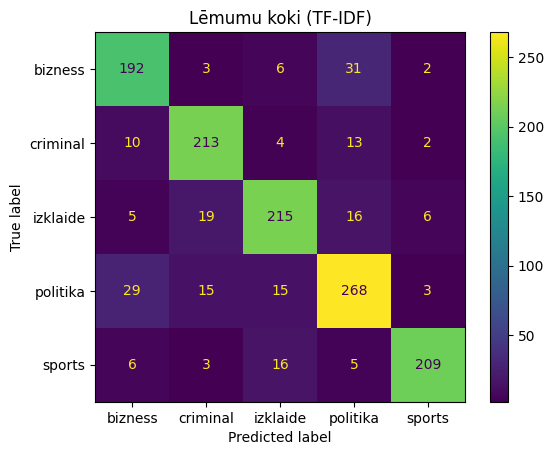
\includegraphics[width=0.75\textwidth]{LemKok_TFIDF}
	\caption{Lēmumu koki - pārpratuma matrica}
	\label{fig:LemKok_TFIDF}
\end{figure}
\begin{table}[H]
\centering
\caption{\label{tab:LemKok}}
\textbf{Lēmumu koku algoritma novērtējums pa kategorijām\\}
\begin{tblr}{
  hlines,
  vlines,
}
kategorija & precizitāte & pārklājums   & F1 mērs \\
bizness  & 0.840517  & 0.833333 & 0.83691      \\
criminal & 0.823529  & 0.867769 & 0.84507       \\
izklaide & 0.848249  & 0.835249 & 0.841699      \\
politika & 0.817365  & 0.827273 & 0.822289      \\
sports   & 0.912281  & 0.870293 & 0.890792      \\
\end{tblr}
\end{table}

\subsection{Konvolūcijas neironu tīkli}
TBD
\begin{figure}[H]
	\centering
	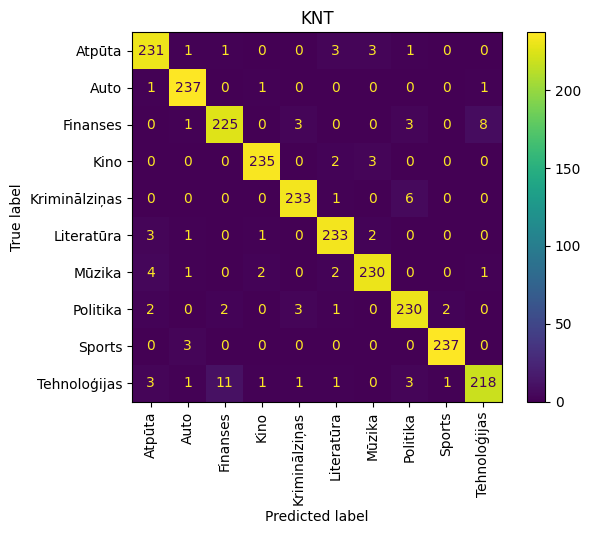
\includegraphics[width=0.75\textwidth]{CNN}
	\caption{Konvolūcijas neironu tīkli - pārpratuma matrica}
	\label{fig:CNN}
\end{figure}

\begin{figure}[H]
	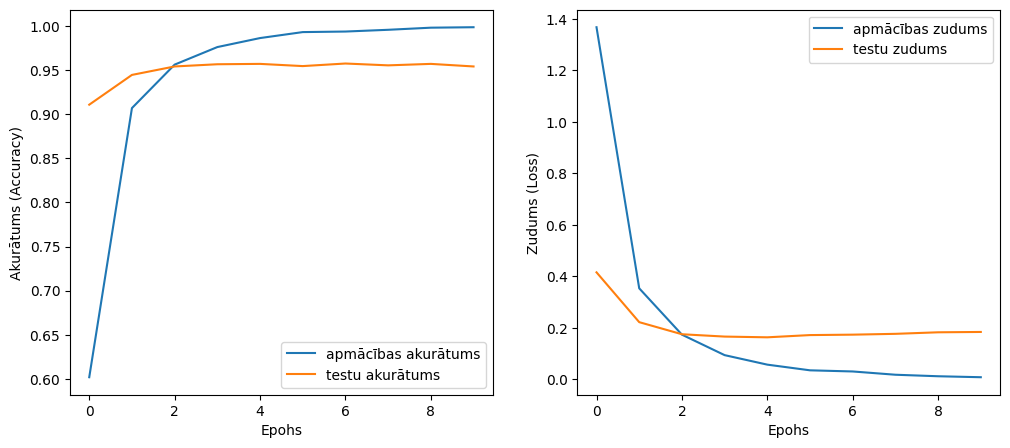
\includegraphics[width=\textwidth]{Accuracy_Loss_CNN_10epoch}
	\caption{Konvolūcijas neironu tīkli - novērtējums pa apmācības posmiem}
	\label{fig:Accuracy_Loss_CNN_10epoch}
\end{figure}

\begin{table}[H]
\centering
\caption{\label{tab:CNN}}
\textbf{Konvolūcijas neironu tīkli - novērtējums pa kategorijām\\}
\begin{tblr}{
  hlines,
  vlines,
}
kategorija & precizitāte & pārklājums   & F1 mērs \\
bizness  & 0.891775  & 0.88412  & 0.887931  \\
criminal & 0.96124   & 0.96124  & 0.96124   \\
izklaide & 0.968     & 0.960317 & 0.964143  \\
politika & 0.920245  & 0.917431 & 0.918836  \\
sports   & 0.958506  & 0.978814 & 0.968553 
\end{tblr}
\end{table}


\section{Modeļu salīdzinājums}
TBD